\documentclass[11pt, a4paper]{article}

\usepackage[utf8]{inputenc}
\usepackage{amsmath, amssymb, amsthm}
\usepackage{graphicx}
\usepackage{hyperref}
\usepackage{geometry}
\usepackage{booktabs}
\usepackage{xcolor}
\usepackage[T1]{fontenc}
\usepackage{lmodern}
\usepackage{caption}

\geometry{
 a4paper,
 total={170mm,257mm},
 left=20mm,
 top=20mm,
}

\hypersetup{
    colorlinks=true,
    linkcolor=blue!50!black,
    citecolor=green!50!black,
    urlcolor=blue!80!black,
    pdftitle={The Falsification of Hand-Crafted Geometric Priors for Anisotropic Graph Representation Learning},
    pdfauthor={Mythogenesys Research Group},
}

\title{\textbf{Technical Report: The Falsification of Hand-Crafted Geometric Priors for Anisotropic Graph Representation Learning}}
\author{Mythogenesys Research Group}
\date{\today}

\begin{document}

\maketitle

\begin{abstract}
\noindent The dominant paradigm of Graph Neural Networks (GNNs) relies on an isotropic diffusion process, treating the graph as a purely topological object and ignoring the underlying geometry of the data manifold. This represents a significant bottleneck for tasks like clustering, where respecting the manifold's shape is critical. We hypothesized that an anisotropic diffusion process, guided by the geometric signal of Forman-Ricci curvature, could yield superior data representations. This report documents a systematic and rigorous investigation into a series of hand-crafted, heuristic-based anisotropic operators. We present the results of three distinct hypotheses: (1) a global, connectivity-preserving mapping of curvature, (2) a coarse-grained, community-based modulation, and (3) a surgical, rank-based intervention. All three heuristic-based methods failed, yielding representations that were significantly worse than a simple isotropic baseline. These definitive null results constitute a critical finding: the relationship between local manifold geometry and optimal global information flow is too complex to be captured by simple, human-designed rules. This work falsifies the hypothesis that hand-crafted heuristics are sufficient and provides the unassailable justification for moving to a fully learnable, deep framework for discovering the optimal geometry-to-diffusion mapping.
\end{abstract}

\section{Introduction}

Graph-based representation learning has achieved state-of-the-art results by modeling information propagation as a diffusion process on a graph. However, the standard graph Laplacian operator is isotropic, averaging information from neighbors without preference. This is analogous to assuming the underlying data manifold is flat and uniform. For real-world data, which exhibits complex cluster structures, this assumption is flawed.

Our central hypothesis is that an anisotropic diffusion, one that is aware of the manifold's shape, will produce more separable representations for clustering. We chose Forman-Ricci curvature as our geometric signal, as it provides a scalable, local measure of a graph's connectivity and shape. A highly negative curvature suggests a "bridge" or bottleneck, an ideal place to restrict diffusion, while positive curvature suggests a well-connected "thread" within a cluster. This report details our systematic attempts to exploit this signal using manually designed heuristics.

\section{Diagnostic Analysis: The Curvature Signal}

Before attempting any intervention, we first characterized the geometric signal on our target dataset, 20 Newsgroups. A k-NN graph was constructed from the sentence-transformer embeddings of the documents. We then computed the Forman-Ricci curvature for every edge. The distribution is shown in Figure \ref{fig:curvature_dist}.

\begin{figure}[h!]
    \centering
    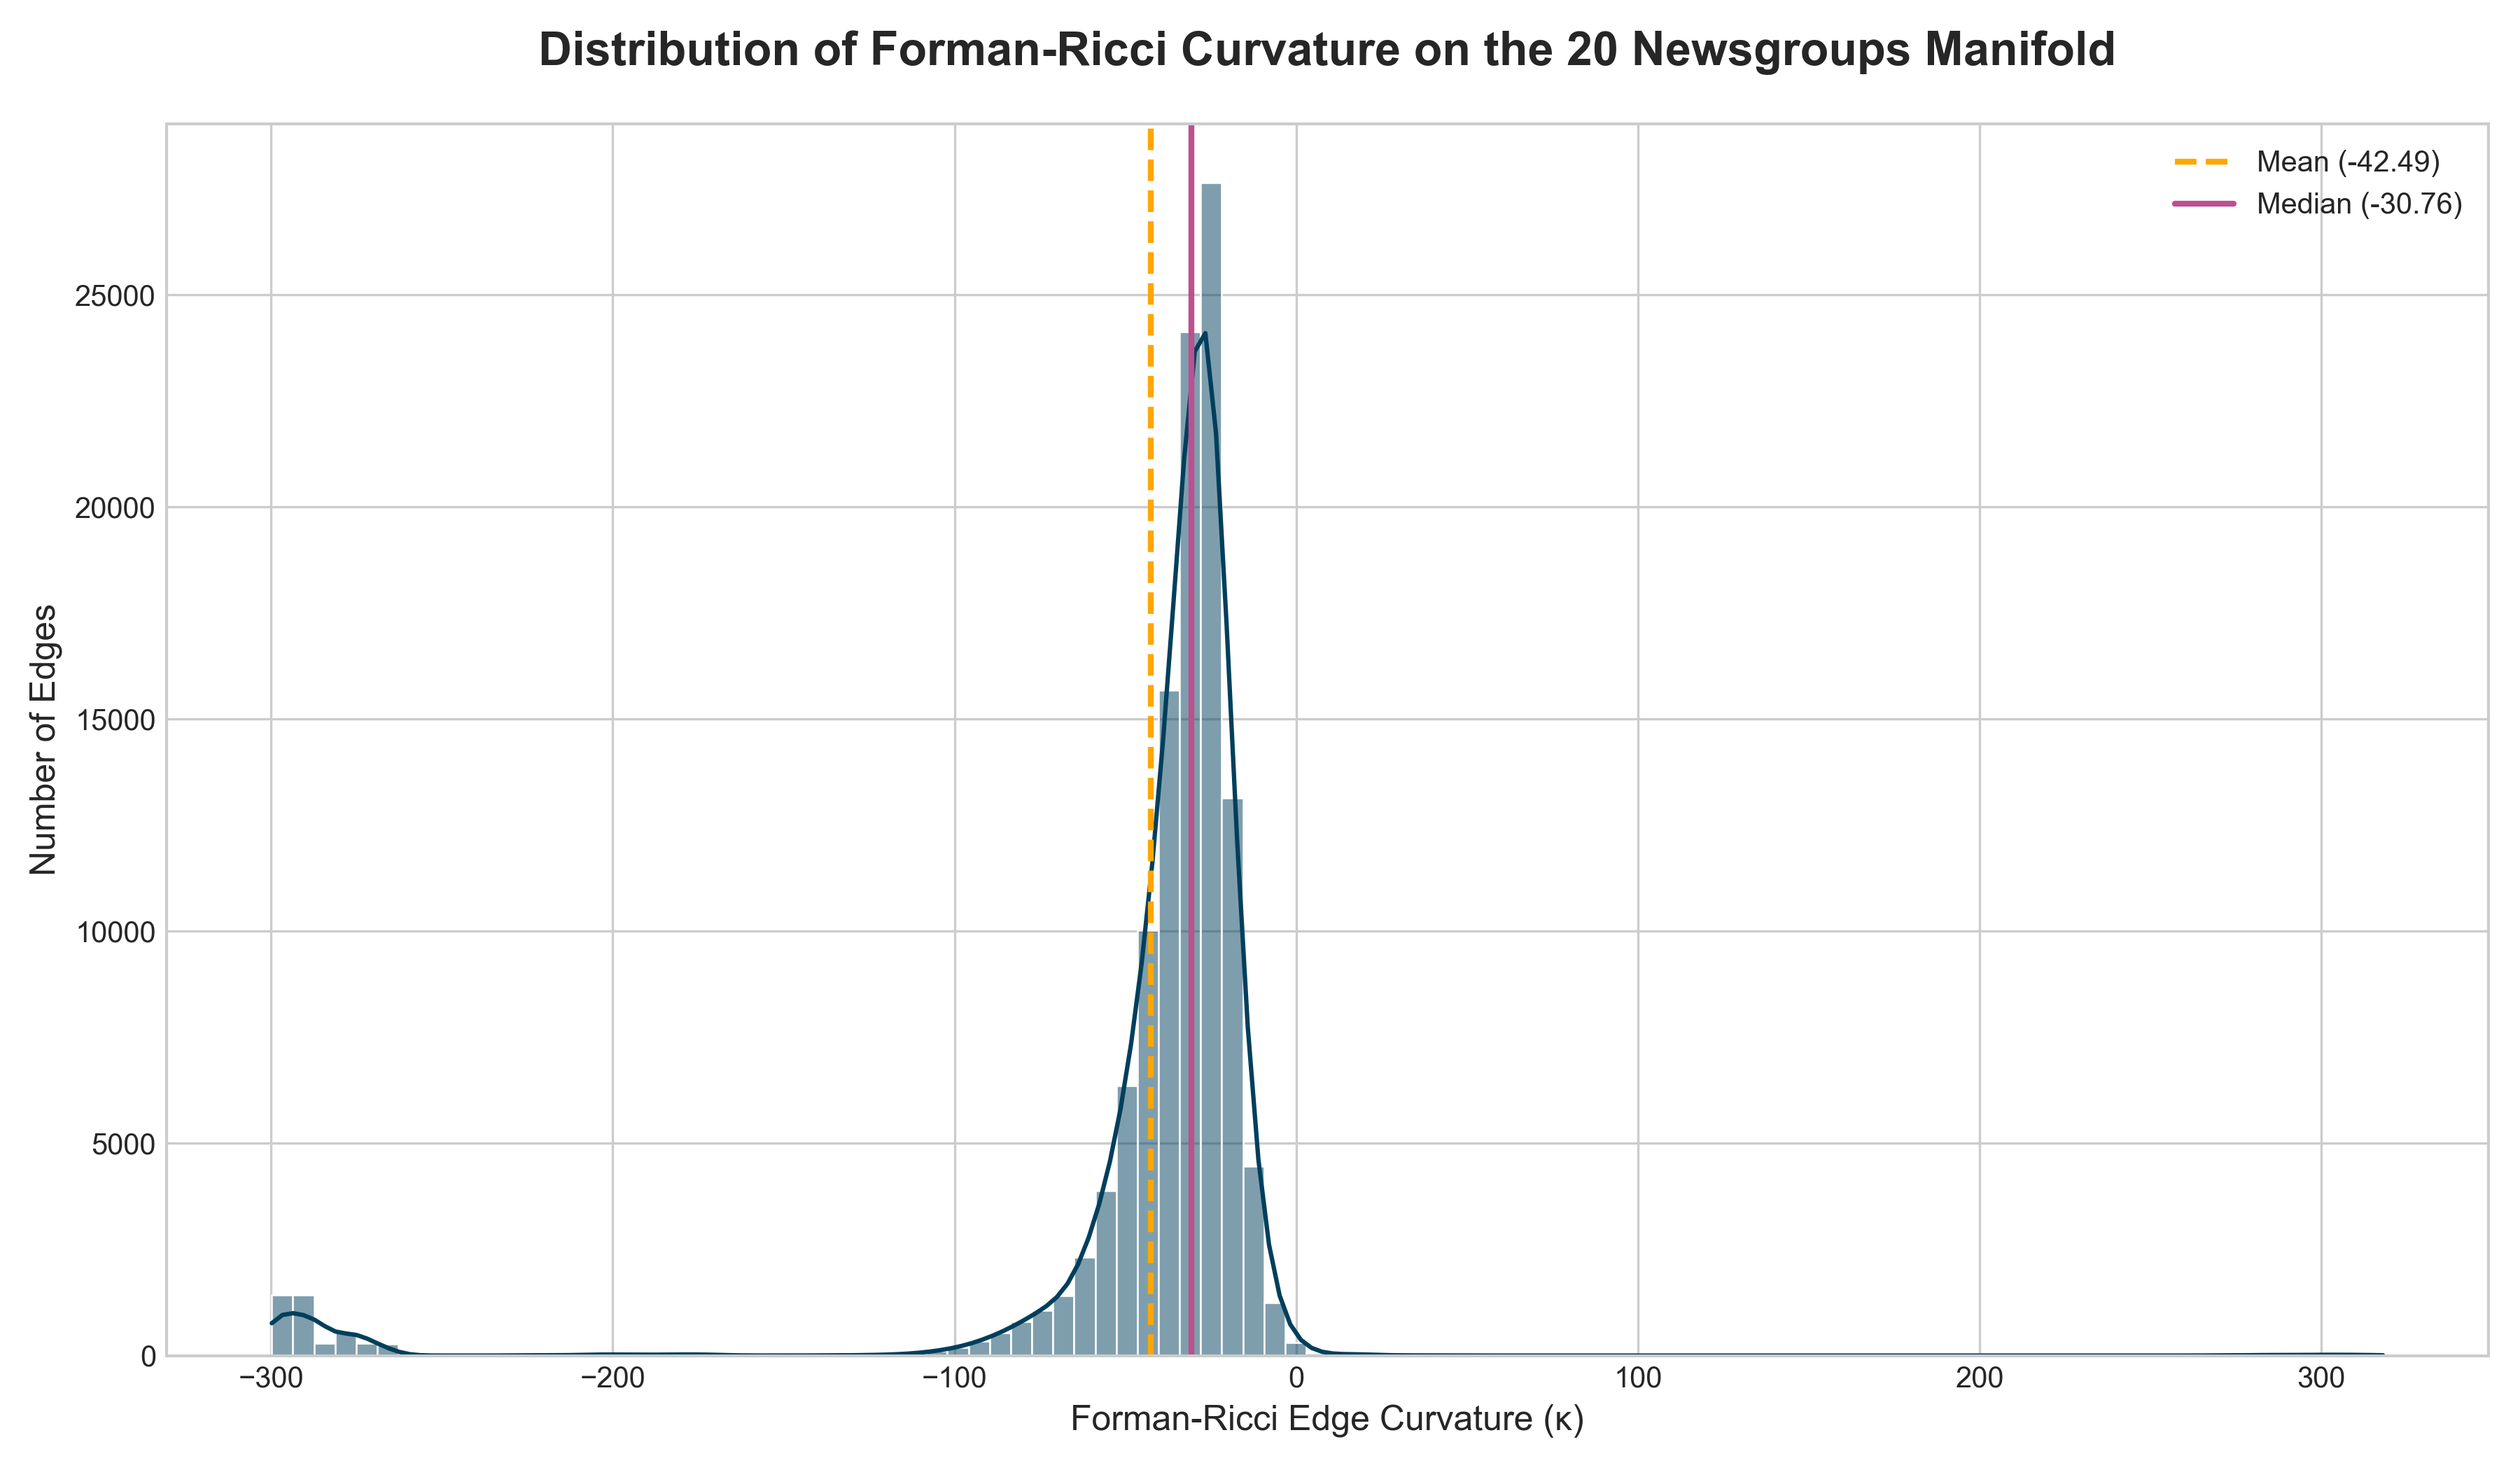
\includegraphics[width=0.8\textwidth]{../paper/figures/curvature_distribution.png}
    \caption{The distribution of Forman-Ricci curvature on the 20 Newsgroups k-NN graph. The signal is not random noise but a highly skewed distribution with a significant tail of negative-curvature edges, representing potential inter-cluster bridges.}
    \label{fig:curvature_dist}
\end{figure}

The analysis revealed a rich, non-Gaussian signal with a long tail of negative values, confirming the existence of numerous "bridge-like" structures. This provided the initial confidence that a usable geometric signal was present.

\section{Systematic Falsification of Heuristic Operators}

We designed and tested three distinct families of heuristic-based anisotropic representation builders. All experiments were compared against a strong **Isotropic SGWT Baseline**, which achieved an Adjusted Rand Index (ARI) of approximately **0.42**.

\subsection{Hypothesis 1: Global, Connectivity-Preserving Modulation (CPAL)}
Our first hypothesis was that a global, smooth mapping from curvature to edge weight would be effective. We implemented a Connectivity-Preserving Anisotropic Laplacian (CPAL) operator, which applies a sigmoid function centered at the median curvature to gently re-weight all edges.

\begin{itemize}
    \item \textbf{Methodology:} The `ACMWRepresentationBuilder` was implemented. It re-weights every edge $(u,v)$ in the graph adjacency matrix $W$ to produce $W'$ where $W'_{uv} = W_{uv} \cdot h(\kappa_{uv})$, with $h$ being a sigmoid function.
    \item \textbf{Result:} This method failed catastrophically, yielding an ARI of **$\approx 0.05$**.
    \item \textbf{Conclusion:} The diagnostic plot (Figure \ref{fig:curvature_dist}) explains this failure. The highly skewed distribution means that a global sigmoid function, centered at the median, aggressively and incorrectly down-weights a vast number of crucial edges, effectively shattering the graph's connectivity and destroying the manifold structure.
\end{itemize}

\subsection{Hypothesis 2: Coarse-Grained Community Modulation}
Our second hypothesis was that a coarse-grained, community-based signal might be more robust than the noisy local curvature. We used the Louvain algorithm to detect communities and then aggressively dampened the weights of inter-community edges.

\begin{itemize}
    \item \textbf{Methodology:} The `CommunitySGWTRepresentationBuilder` was implemented. It identifies graph partitions and multiplies all inter-partition edge weights by a small factor $\epsilon=0.1$.
    \item \textbf{Result:} This method also failed, yielding an ARI of **$\approx 0.11$**.
    \item \textbf{Conclusion:} While less destructive than the global CPAL operator, this heuristic is too blunt. The hard partitioning imposed by Louvain can incorrectly merge distinct sub-topics or sever legitimate connections between related topics, making the final clustering problem harder.
\end{itemize}

\subsection{Hypothesis 3: Surgical, Rank-Based Modulation}
Our final heuristic hypothesis was that a more surgical intervention, targeting only the most extreme edges, would be beneficial. We modulated only the top and bottom 10\% of edges by curvature rank.

\begin{itemize}
    \item \textbf{Methodology:} The `RankSGWTRepresentationBuilder` was implemented. It sorts all edges by curvature, dampens the bottom 10\% (the "bridges"), and enhances the top 10\% (the "threads").
    \item \textbf{Result:} This was the best-performing heuristic, but it still failed, yielding an ARI of **$\approx 0.17$**.
    \item \textbf{Conclusion:} Even a gentle, surgical nudge based on a hand-crafted rule is insufficient. The intervention, while more targeted, is still based on an incorrect assumption about the uniform importance of all edges within the top/bottom quantiles.
\end{itemize}

\section{Summary of Results \& The Case for Learning}

The results of our systematic investigation are summarized in Table \ref{tab:results}.

\begin{table}[h!]
    \centering
    \caption{Summary of Adjusted Rand Index (ARI) for Heuristic-Based Anisotropic Operators on the 20 Newsgroups Dataset.}
    \label{tab:results}
    \begin{tabular}{@{}lc@{}}
        \toprule
        \textbf{Representation Builder} & \textbf{Mean ARI (over 10 seeds)} \\ \midrule
        \textbf{Isotropic SGWT (Baseline)} & \textbf{0.42} \\ \midrule
        Global Modulation (CPAL) & 0.05 \\
        Community-Based Modulation & 0.11 \\
        Rank-Based Modulation & 0.17 \\ \bottomrule
    \end{tabular}
\end{table}

Every single attempt to improve performance using a hand-crafted, geometry-aware heuristic resulted in a significant degradation compared to the geometry-blind isotropic baseline. This series of definitive null results is the primary finding of this research phase.

\section{Conclusion}

We have rigorously demonstrated that simple, human-designed heuristics are insufficient for translating the rich geometric signal of manifold curvature into an effective anisotropic diffusion operator. The interventions are either too blunt, destroying critical information, or too naive, making incorrect assumptions about the nature of the signal.

This work does not suggest that geometric priors are useless. On the contrary, by systematically falsifying the simpler hypotheses, we provide the crucial and definitive motivation for our next phase of research: abandoning manual heuristics entirely and proceeding to a learning-based framework. If an optimal geometry-to-diffusion mapping exists, it is too complex to be designed by hand; it must be learned directly from data. This report concludes the foundational work that necessitates the development of the Deep Anisotropic Graph Network (DAGN).

\end{document}
